% Copyright (c) 2021 Robert Carnell

\documentclass[11pt,letter]{book}

\usepackage[T1]{fontenc}

% Fonts added for the book
\usepackage[bitstream-charter]{mathdesign} % use the bitstream-charter True Type font

% ---- Gramps Packages ----
%\usepackage[latin1]{inputenc}%
\usepackage[latin1,utf8]{inputenc}%
\usepackage{graphicx}% Extended graphics support
\usepackage{longtable}% For multi-page tables
\usepackage{calc}% For some calculations
\usepackage{ifthen}% For table width calculations
\usepackage{ragged2e}% For left aligning with hyphenation
\usepackage{wrapfig}% wrap pictures in text

% Packages added for the book
\usepackage[all]{genealogytree} % genealogy-tree package for trees
\usepackage[hidelinks]{hyperref} % to break long URL lines, and make TOC clickable
%\usepackage{draftwatermark} % create draft watermark
%\SetWatermarkText{DRAFT}
%\SetWatermarkScale{1}

% --------- Gramps Section ----------

% Depending on your LaTeX installation, the margins may be too
% narrow.  This can be corrected by uncommenting the following
% two lines and adjusting the width appropriately. The example
% removes 0.5in from each margin. (Adds 1 inch to the text)
%\addtolength{\oddsidemargin}{-0.5in}%
%\addtolength{\textwidth}{1.0in}%

% Vertical spacing between paragraphs:
% take one of three possibilities or modify to your taste:
\setlength{\parskip}{1.0ex plus0.2ex minus0.2ex}%
%\setlength{\parskip}{1.5ex plus0.3ex minus0.3ex}%
%\setlength{\parskip}{2.0ex plus0.4ex minus0.4ex}%

% Vertical spacing between lines:
% take one of three possibilities or modify to your taste:
\renewcommand{\baselinestretch}{1.0}%
%\renewcommand{\baselinestretch}{1.1}%
%\renewcommand{\baselinestretch}{1.2}%

% Indentation; substitute for '1cm' of gramps, 2.5em is right for 12pt
% take one of three possibilities or modify to your taste:
\newlength{\grbaseindent}%
%\setlength{\grbaseindent}{3.0em}%
\setlength{\grbaseindent}{2.5em}%
%\setlength{\grbaseindent}{2.0em}%


% -------------------------------------------------------------
% New lengths, counters and commands for calculations in tables
% -------------------------------------------------------------

\newlength{\grtabwidth}%
\newlength{\grtabprepos}%
\newlength{\grreqwidth}%
\newlength{\grtempwd}%
\newlength{\grmaxwidth}%
\newlength{\grprorated}%
\newlength{\grxwd}%
\newlength{\grwidthused}%
\newlength{\grreduce}%
\newlength{\grcurcolend}%
\newlength{\grspanwidth}%
\newlength{\grleadlabelwidth}%
\newlength{\grminpgindent}%
\newlength{\grlistbacksp}%
\newlength{\grpictsize}%
\newlength{\grmaxpictsize}%
\newlength{\grtextsize}%
\newlength{\grmaxtextsize}%
\newcounter{grtofixcnt}%
\newcounter{grxwdcolcnt}%
%
%
\newcommand{\grinitlength}[2]{%
  \ifthenelse{\isundefined{#1}}%
    {\newlength{#1}}{}%
  \setlength{#1}{#2}%
}%
%
\newcommand{\grinittab}[2]{%    #1: tabwidth, #2 = 1.0/anz-cols
  \setlength{\grtabwidth}{#1}%
  \setlength{\grprorated}{#2\grtabwidth}%
  \setlength{\grwidthused}{0em}%
  \setlength{\grreqwidth}{0em}%
  \setlength{\grmaxwidth }{0em}%
  \setlength{\grxwd}{0em}%
  \setlength{\grtempwd}{0em}%
  \setlength{\grpictsize}{0em}%
  \setlength{\grmaxpictsize}{0em}%
  \setlength{\grtextsize}{0em}%
  \setlength{\grmaxtextsize}{0em}%
  \setlength{\grcurcolend}{0em}%
  \setcounter{grxwdcolcnt}{0}%
  \setcounter{grtofixcnt}{0}%  number of wide cols%
  \grinitlength{\grcolbega}{0em}% beg of first col
}%
%
\newcommand{\grmaxvaltofirst}[2]{%
  \ifthenelse{\lengthtest{#1 < #2}}%
    {\setlength{#1}{#2}}{}%
}%
%
\newcommand{\grsetreqfull}{%
  \grmaxvaltofirst{\grmaxpictsize}{\grpictsize}%
  \grmaxvaltofirst{\grmaxtextsize}{\grtextsize}%
}%
%
\newcommand{\grsetreqpart}[1]{%
  \addtolength{\grtextsize}{#1 - \grcurcolend}%
  \addtolength{\grpictsize}{#1 - \grcurcolend}%
  \grsetreqfull%
}%
%
\newcommand{\grdividelength}{%
 \setlength{\grtempwd}{\grtabwidth - \grwidthused}%
%    rough division of lengths:
%    if 0 < #1 <= 10: \grxwd = ~\grtempwd / grtofixcnt
%    otherwise: \grxwd =  \grprorated
 \ifthenelse{\value{grtofixcnt} > 0}%
  {\ifthenelse{\value{grtofixcnt}=1}%
                    {\setlength{\grxwd}{\grtempwd}}{%
    \ifthenelse{\value{grtofixcnt}=2}
                    {\setlength{\grxwd}{0.5\grtempwd}}{%
     \ifthenelse{\value{grtofixcnt}=3}
                    {\setlength{\grxwd}{0.333\grtempwd}}{%
      \ifthenelse{\value{grtofixcnt}=4}
                    {\setlength{\grxwd}{0.25\grtempwd}}{%
       \ifthenelse{\value{grtofixcnt}=5}
                    {\setlength{\grxwd}{0.2\grtempwd}}{%
        \ifthenelse{\value{grtofixcnt}=6}
                    {\setlength{\grxwd}{0.166\grtempwd}}{%
         \ifthenelse{\value{grtofixcnt}=7}
                    {\setlength{\grxwd}{0.143\grtempwd}}{%
          \ifthenelse{\value{grtofixcnt}=8}
                    {\setlength{\grxwd}{0.125\grtempwd}}{%
           \ifthenelse{\value{grtofixcnt}=9}
                    {\setlength{\grxwd}{0.111\grtempwd}}{%
            \ifthenelse{\value{grtofixcnt}=10}
                    {\setlength{\grxwd}{0.1\grtempwd}}{%
             \setlength{\grxwd}{\grprorated}% give up, take \grprorated%
    }}}}}}}}}}%
  \setlength{\grreduce}{0em}%
  }{\setlength{\grxwd}{0em}}%
}%
%
\newcommand{\grtextneedwidth}[1]{%
  \settowidth{\grtempwd}{#1}%
  \grmaxvaltofirst{\grtextsize}{\grtempwd}%
}%
%
\newcommand{\grcolsfirstfix}[5]{%
  \grinitlength{#1}{\grcurcolend}%
  \grinitlength{#3}{0em}%
  \grinitlength{#4}{\grmaxpictsize}%
  \grinitlength{#5}{\grmaxtextsize}%
  \grinitlength{#2}{#5}%
  \grmaxvaltofirst{#2}{#4}%
  \addtolength{#2}{2\tabcolsep}%
  \grmaxvaltofirst{\grmaxwidth}{#2}%
  \ifthenelse{\lengthtest{#2 < #4} \or \lengthtest{#2 < \grprorated}}%
    { \setlength{#3}{#2}%
      \addtolength{\grwidthused}{#2} }%
    { \stepcounter{grtofixcnt} }%
  \addtolength{\grcurcolend}{#2}%
}%
%
\newcommand{\grcolssecondfix}[4]{%
  \ifthenelse{\lengthtest{\grcurcolend < \grtabwidth}}%
    { \setlength{#3}{#2} }%
    { \addtolength{#1}{-\grreduce}%
      \ifthenelse{\lengthtest{#2 = \grmaxwidth}}%
        { \stepcounter{grxwdcolcnt}}%
        { \ifthenelse{\lengthtest{#3 = 0em} \and %
                       \lengthtest{#4 > 0em}}%
            { \setlength{\grtempwd}{#4}%
              \grmaxvaltofirst{\grtempwd}{\grxwd}%
              \addtolength{\grreduce}{#2 - \grtempwd}%
              \setlength{#2}{\grtempwd}%
              \addtolength{\grwidthused}{#2}%
              \addtocounter{grtofixcnt}{-1}%
              \setlength{#3}{#2}%
            }{}%
        }%
    }%
}%
%
\newcommand{\grcolsthirdfix}[3]{%
  \ifthenelse{\lengthtest{\grcurcolend < \grtabwidth}}%
    {}{ \addtolength{#1}{-\grreduce}%
        \ifthenelse{\lengthtest{#3 = 0em} \and %
                     \lengthtest{#2 < \grmaxwidth}}%
          { \ifthenelse{\lengthtest{#2 < 0.5\grmaxwidth}}%
              { \setlength{\grtempwd}{0.5\grxwd}%
                \grmaxvaltofirst{\grtempwd}{0.7\grprorated}}%
              { \setlength{\grtempwd}{\grxwd}}%
            \addtolength{\grreduce}{#2 - \grtempwd}%
            \setlength{#2}{\grtempwd}%
            \addtolength{\grwidthused}{#2}%
            \addtocounter{grtofixcnt}{-1}%
            \setlength{#3}{#2}%
          }{}%
      }%
}%
%
\newcommand{\grcolsfourthfix}[3]{%
  \ifthenelse{\lengthtest{\grcurcolend < \grtabwidth}}%
    {}{ \addtolength{#1}{-\grreduce}%
        \ifthenelse{\lengthtest{#3 = 0em}}%
          { \addtolength{\grreduce}{#2 - \grxwd}%
            \setlength{#2}{\grxwd}%
            \setlength{#3}{#2}%
          }{}%
      }%
}%
%
\newcommand{\grgetspanwidth}[4]{%
  \grinitlength{#1}{#3 - #2 + #4}%
}%
%
\newcommand{\tabheadstrutceil}{%
  \rule[0.0ex]{0.00em}{3.5ex}}%
\newcommand{\tabheadstrutfloor}{%
  \rule[-2.0ex]{0.00em}{2.5ex}}%
\newcommand{\tabrowstrutceil}{%
  \rule[0.0ex]{0.00em}{2.9ex}}%
\newcommand{\tabrowstrutfloor}{%
  \rule[-0.1ex]{0.00em}{2.0ex}}%
%
\newcommand{\grempty}[1]{}%
%
\newcommand{\graddvdots}[1]{%
  \hspace*{\fill}\hspace*{\fill}\raisebox{#1}{\vdots}%
}%
%
\newcommand{\grtabpgbreak}[4]{%
  #1 { \parbox[t]{ #2 - 2\tabcolsep}{\tabheadstrutceil\hspace*{\fill}%
  \raisebox{#4}{\vdots} #3{#4} \hspace*{\fill}\tabheadstrutfloor}}%
}%
%
\newcommand{\grcolpart}[3]{%
  #1 { \parbox[t]{ #2 - 2\tabcolsep}%
  {\tabrowstrutceil #3~\\[-1.6ex]\tabrowstrutfloor}}%
}%
%
\newcommand{\grminpghead}[2]{%
  \setlength{\grminpgindent}{#1\grbaseindent-\grlistbacksp}%
  \hspace*{\grminpgindent}%
  \ifthenelse{\not \lengthtest{#2em > 0em}}%
    {\begin{minipage}[t]{\textwidth -\grminpgindent}}%
    {\begin{minipage}[t]{\textwidth -\grminpgindent%
        -#2\grbaseindent -4\tabcolsep}}%
}%
%
\newcommand{\grminpgtail}{%
  \end{minipage}\parindent0em%
}%
%
\newcommand{\grlisthead}[1]{%
  \begin{list}{#1}%
    { \setlength{\labelsep}{0.5em}%
      \setlength{\labelwidth}{\grleadlabelwidth}%
      \setlength{\leftmargin}{\grlistbacksp}%
    }\item%
}%
%
\newcommand{\grlisttail}{%
  \end{list}%
}%
%
\newcommand{\grprepleader}[1]{%
  \settowidth{\grtempwd}{#1}%
  \ifthenelse{\lengthtest{\grtempwd > \grleadlabelwidth}}%
    { \setlength{\grleadlabelwidth}{\grtempwd}}{}%
  \setlength{\grlistbacksp}{\grleadlabelwidth + 1.0em}%
}%
%
\newcommand{\grprepnoleader}{%
  \setlength{\grleadlabelwidth}{0em}%
  \setlength{\grlistbacksp}{0em}%
}%
%
\newcommand{\grmkpicture}[4]{%
    \begin{wrapfigure}{r}{#2\grbaseindent}%
      \vspace{-6ex}%
      \begin{center}%
      \includegraphics[%
        width= #2\grbaseindent,%
        height= #3\grbaseindent,%
          keepaspectratio]%
        {#1}\\%
      {\RaggedRight\footnotesize#4}%
      \end{center}%
    \end{wrapfigure}%
    \settowidth{\grtempwd}{\footnotesize#4}%
    \setlength{\grxwd}{#2\grbaseindent}%
    \ifthenelse{\lengthtest{\grtempwd < 0.7\grxwd}}%
                    {\setlength{\grxwd}{1ex}}{%
      \ifthenelse{\lengthtest{\grtempwd < 1.2\grxwd}}%
                    {\setlength{\grxwd}{2ex}}{%
        \ifthenelse{\lengthtest{\grtempwd < 1.8\grxwd}}%
                    {\setlength{\grxwd}{6ex}}{%
          \ifthenelse{\lengthtest{\grtempwd < 2.0\grxwd}}%
                    {\setlength{\grxwd}{10ex}}{%
                     \setlength{\grxwd}{12ex}}%
                    }}}%
  \setlength{\grtempwd}{#3\grbaseindent + \grxwd}%
  \rule[-\grtempwd]{0pt}{\grtempwd}%
  \setlength{\grtabprepos}{-\grtempwd}%
}%

% -------------------- End Gramps Section ----------------------

\title{\bf Carnell-Rettgers Family Genealogy \\
       \large Volume III - Rettgers / Hartenstine / Bechtel / Fett}
\author{Robert Carnell}
\date{\today}

\begin{document}
\frontmatter
\maketitle
\clearpage

\begingroup
\parindent 0pt
\parskip
\baselineskip
Copyright \textcopyright{} 2021 Robert Carnell

All rights reserved.  This book or any portion thereof may not be reproduced or used in any manner whatsoever with the express written permission of the author except for the use or brief quotations in a book review or genealogical research.
\endgroup
\clearpage

\tableofcontents
\mainmatter

\chapter{Introduction}

The Rettgers, Hartenstine, Bechtel, and Fett family lines are primarily of Western European origin.  It consists of Palatines, Huguenots, and other refugees from European religious persecution.  One line of the family, the Wynne's, accompanied William Penn to America from England in 1682.  The most recent immigration occurred with the Roettgers family in the second half of the 1800s.

\chapter{Ancestors of Ithamar Benedict Rettgers}

\section{Tree}

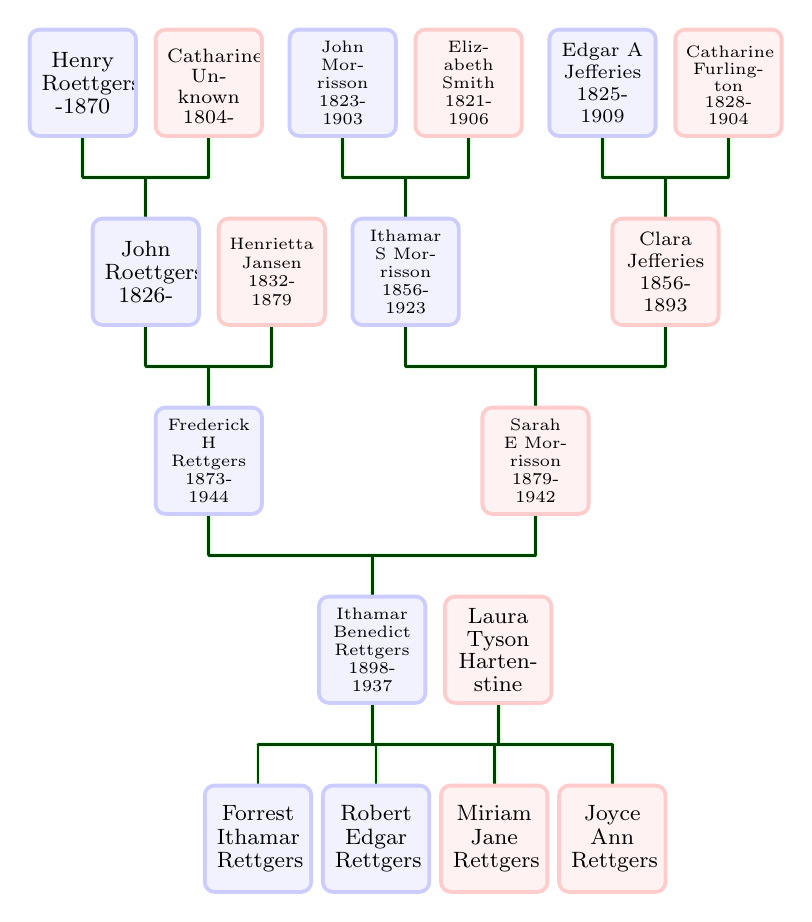
\begin{tikzpicture}
	\genealogytree[
		template=signpost, 
		node size=1.4cm, 
		level size=1.4cm,
		tcbset={male/.style={colframe=blue!20, colback=blue!5},
			female/.style={colframe=red!20, colback=red!5}},
		box={fit basedim=8pt, boxsep=2pt, no shadow}
	]{
		parent{
			c[male]{Forrest Ithamar Rettgers}
			g[male]{Robert Edgar Rettgers}
			c[female]{Miriam Jane Rettgers}
			c[female]{Joyce Ann Rettgers}
			parent{
				g[male]{Ithamar Benedict Rettgers\\1898-1937}
				parent{
					g[male]{Frederick H Rettgers\\1873-1944}
					parent{
						g[male]{John Roettgers\\1826-}
						parent{
							g[male]{Henry Roettgers\\-1870}
						}
						parent{
							g[female]{Catharine Unknown\\1804-}
						}
					}
					parent{
						g[female]{Henrietta Jansen\\1832-1879}
					}
				}
				parent{
					g[female]{Sarah E Morrisson\\1879-1942}
					parent{
						g[male]{Ithamar S Morrisson\\1856-1923}
						parent{
							g[male]{John Morrisson\\1823-1903}
						}
						parent{
							g[female]{Elizabeth Smith\\1821-1906}
						}
					}
					parent{
						g[female]{Clara Jefferies\\1856-1893}
						parent{
							g[male]{Edgar A Jefferies\\1825-1909}
						}
						parent{
							g[female]{Catharine Furlington\\1828-1904}
						}
					}
				}
			}
			parent{
				g[female]{Laura Tyson Hartenstine}
			}
		}
	}
\end{tikzpicture}

\section{Genealogy}

\input{../tex_output/det_ancestor_report_Rettgers_mod.tex}

\chapter{Ancestors of Laura Tyson Hartenstine}

\section{Tree}

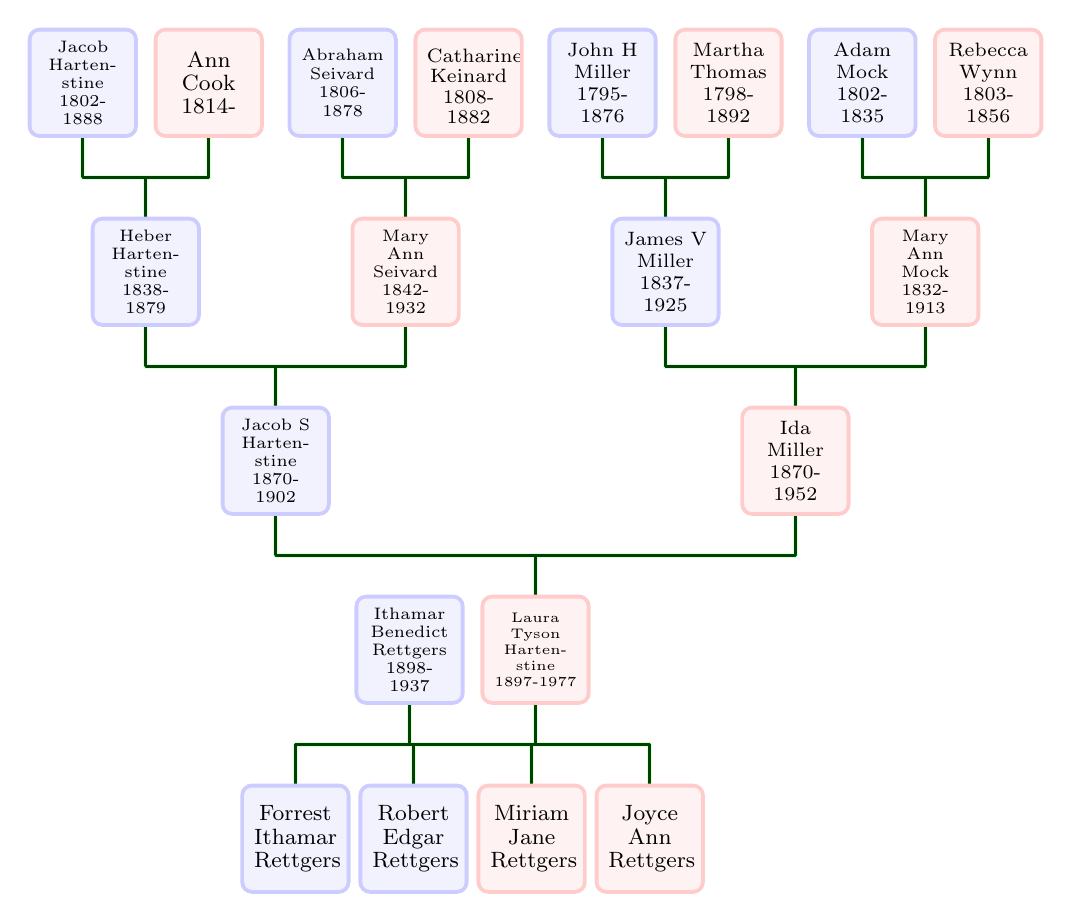
\begin{tikzpicture}
	\genealogytree[
		template=signpost, 
		node size=1.4cm, 
		level size=1.4cm,
		tcbset={male/.style={colframe=blue!20, colback=blue!5},
			female/.style={colframe=red!20, colback=red!5}},
		box={fit basedim=8pt, boxsep=2pt, no shadow}
	]{
		parent{
			c[male]{Forrest Ithamar Rettgers}
			g[male]{Robert Edgar Rettgers}
			c[female]{Miriam Jane Rettgers}
			c[female]{Joyce Ann Rettgers}
			parent{
				g[male]{Ithamar Benedict Rettgers\\1898-1937}
			}
			parent{
				g[female]{Laura Tyson Hartenstine\\1897-1977}
				parent{
					g[male]{Jacob S Hartenstine\\1870-1902}
					parent{
						g[male]{Heber Hartenstine\\1838-1879}
						parent{
							g[male]{Jacob Hartenstine\\1802-1888}
						}
						parent{
							g[female]{Ann Cook\\1814-}
						}
					}
					parent{
						g[female]{Mary Ann Seivard\\1842-1932}
						parent{
							g[male]{Abraham Seivard\\1806-1878}
						}
						parent{
							g[female]{Catharine Keinard\\1808-1882}
						}
					}
				}
				parent{
					g[female]{Ida Miller\\1870-1952}
					parent{
						g[male]{James V Miller\\1837-1925}
						parent{
							g[male]{John H Miller\\1795-1876}
						}
						parent{
							g[female]{Martha Thomas\\1798-1892}
						}
					}
					parent{
						g[female]{Mary Ann Mock\\1832-1913}
						parent{
							g[male]{Adam Mock\\1802-1835}
						}
						parent{
							g[female]{Rebecca Wynn\\1803-1856}
						}
					}
				}
			}
		}
	}
\end{tikzpicture}

\section{Genealogy}

\input{../tex_output/det_ancestor_report_Hartenstine_mod.tex}

\chapter{Ancestors of Floyd William Fett}

\section{Tree}

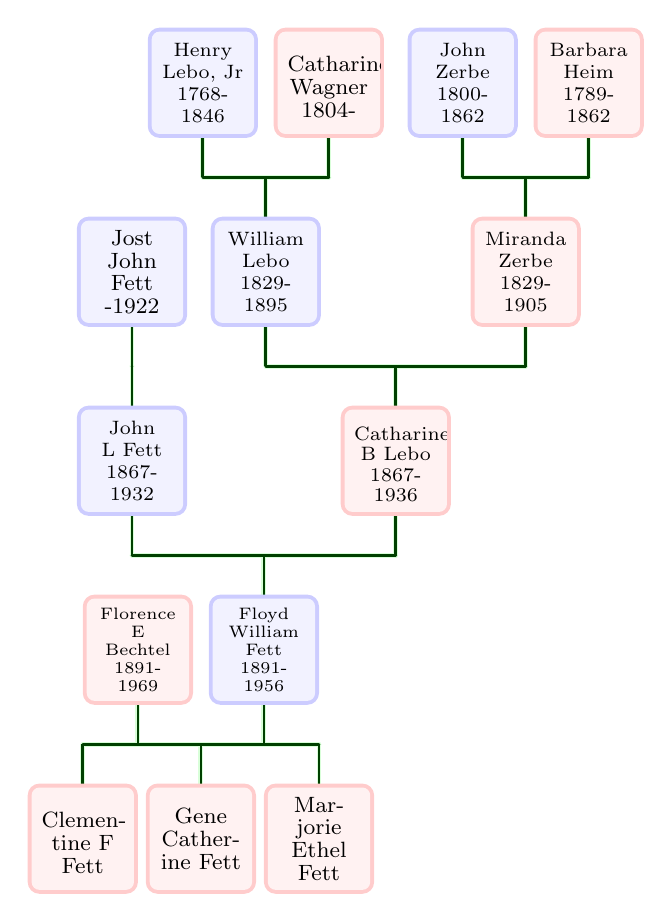
\begin{tikzpicture}
	\genealogytree[
		template=signpost, 
		node size=1.4cm, 
		level size=1.4cm,
		tcbset={male/.style={colframe=blue!20, colback=blue!5},
			female/.style={colframe=red!20, colback=red!5}},
		box={fit basedim=8pt, boxsep=2pt, no shadow}
	]{
		parent{
			c[female]{Clementine F Fett}
			c[female]{Gene Catherine Fett}
			g[female]{Marjorie Ethel Fett}
			parent{
				g[female]{Florence E Bechtel\\1891-1969}
			}
			parent{
				g[male]{Floyd William Fett\\1891-1956}
				parent{
					g[male]{John L Fett\\1867-1932}
					parent{
						g[male]{Jost John Fett\\-1922}
					}
				}
				parent{
					g[female]{Catharine B Lebo\\1867-1936}
					parent{
						g[male]{William Lebo\\1829-1895}
						parent{
							g[male]{Henry Lebo, Jr\\1768-1846}
						}
						parent{
							g[female]{Catharine Wagner\\1804-}
						}
					}
					parent{
						g[female]{Miranda Zerbe\\1829-1905}
						parent{
							g[male]{John Zerbe\\1800-1862}
						}
						parent{
							g[female]{Barbara Heim\\1789-1862}
						}
					}
				}
			}
		}
	}
\end{tikzpicture}

\section{Genealogy}

\input{../tex_output/det_ancestor_report_Fett_mod.tex}

\chapter{Ancestors of Florence Ethel Bechtel}

\section{Tree}

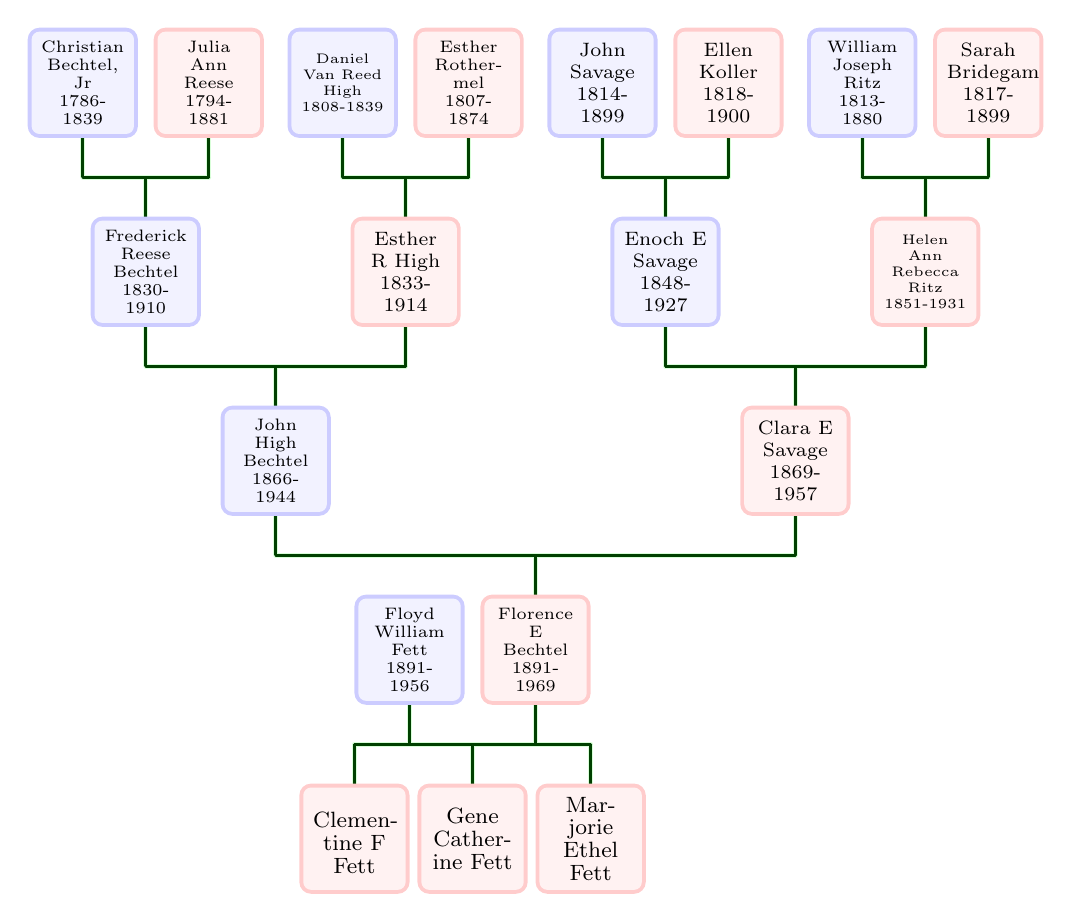
\begin{tikzpicture}
	\genealogytree[
		template=signpost, 
		node size=1.4cm, 
		level size=1.4cm,
		tcbset={male/.style={colframe=blue!20, colback=blue!5},
			female/.style={colframe=red!20, colback=red!5}},
		box={fit basedim=8pt, boxsep=2pt, no shadow}
	]{
		parent{
			c[female]{Clementine F Fett}
			c[female]{Gene Catherine Fett}
			g[female]{Marjorie Ethel Fett}
			parent{
				g[male]{Floyd William Fett\\1891-1956}
			}
			parent{
				g[female]{Florence E Bechtel\\1891-1969}
				parent{
					g[male]{John High Bechtel\\1866-1944}
					parent{
						g[male]{Frederick Reese Bechtel\\1830-1910}
						parent{
							g[male]{Christian Bechtel, Jr\\1786-1839}
						}
						parent{
							g[female]{Julia Ann Reese\\1794-1881}
						}
					}
					parent{
						g[female]{Esther R High\\1833-1914}
						parent{
							g[male]{Daniel Van Reed High\\1808-1839}
						}
						parent{
							g[female]{Esther Rothermel\\1807-1874}
						}
					}
				}
				parent{
					g[female]{Clara E Savage\\1869-1957}
					parent{
						g[male]{Enoch E Savage\\1848-1927}
						parent{
							g[male]{John Savage\\1814-1899}
						}
						parent{
							g[female]{Ellen Koller\\1818-1900}
						}
					}
					parent{
						g[female]{Helen Ann Rebecca Ritz\\1851-1931}
						parent{
							g[male]{William Joseph Ritz\\1813-1880}
						}
						parent{
							g[female]{Sarah Bridegam\\1817-1899}
						}
					}
				}

			}
		}
	}
\end{tikzpicture}

\section{Genealogy}

\input{../tex_output/det_ancestor_report_Bechtel_mod.tex}

\chapter{Endnotes}

\section{Rettgers Endnotes}

\footnotesize

\input{../tex_output/det_ancestor_report_Rettgers_mod_notes.tex}

\normalsize

\section{Hartenstine Endnotes}

\footnotesize

\input{../tex_output/det_ancestor_report_Hartenstine_mod_notes.tex}

\normalsize

\section{Fett Endnotes}

\footnotesize

\input{../tex_output/det_ancestor_report_Fett_mod_notes.tex}

\normalsize

\section{Bechtel Endnotes}

\footnotesize

\input{../tex_output/det_ancestor_report_Bechtel_mod_notes.tex}

\normalsize

\end{document}
